Chokers are curb extensions at midblock locations that narrow a street by ultimately creating wider sidewalks. They are also known as safe crosses when marked as crosswalks. Chokers can be made by widening one side of the curb or by bringing both curbs in, giving it the “pinch point” along the street (See \figref{choker}). The main purpose of chokers is to decrease speed of incoming vehicles at a mid-point along the streets, create a seamless transition between a commercial and a residential area, and to narrow exceedingly wide intersections \cite{walking-info-chokers}.

\begin{figure}[h]
\centering
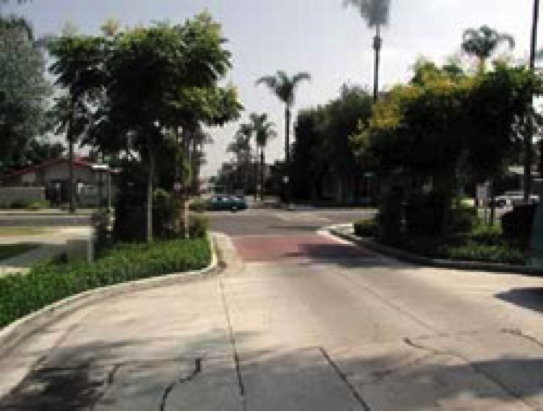
\includegraphics[scale=1]{choker.png}
\caption[Choker]{This choker requires drivers to yield upon entering}\label{fig:choker}
\end{figure}

Two-lane chokers (See \figref{two-lane-choker}) leave two lanes in the street cross section narrower than the width of a normal cross section, while one-lane chokers narrow the width to allow travel in only one direction at a time. These chokers are effective for areas with substantial speed problems and streets with minimum or no parking on-site.

\begin{figure}
\centering
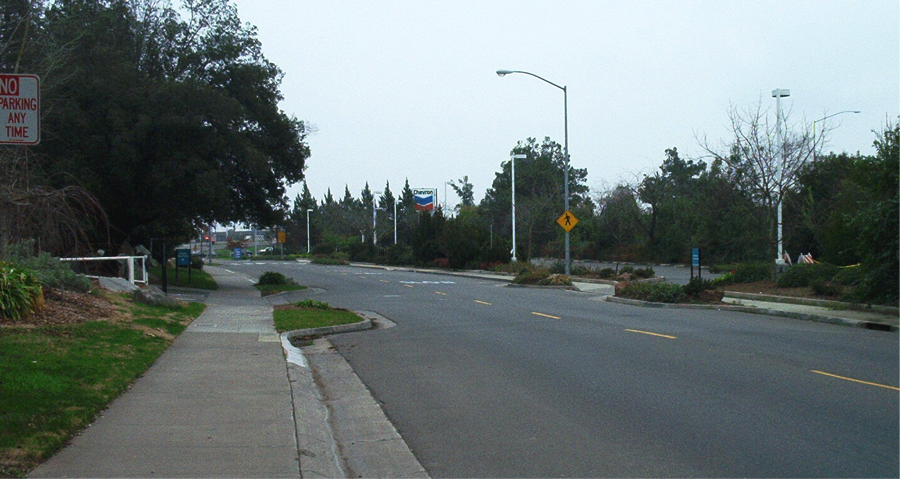
\includegraphics[scale=1]{two-lane-choker.png}
\caption{Two-Lane Chokers}\label{fig:two-lane-choker}
\end{figure}

\subsubsection{Advantages and Disadvantages}

The various advantages of chokers are:\begin{itemize}
\item ability to reduce both speed and volume significantly
\item easily negotiable by large vehicles (for example, fire trucks)
\item improving aesthetic value when well designed
\end{itemize}

The disadvantages include:\begin{itemize}
\item Eliminates on-street parking
\item Requires bicyclists to briefly merge with vehicular traffic
\item Absence of vertical or horizontal deflation limiting the effect of chokers on vehicle speed.
\end{itemize}

\subsubsection{Effectiveness}

Chokers can ultimately increase the visibility of pedestrians as well as to reduce pedestrian crossing width, while the speed of vehicles is reduced by 4 percent on average for two-lane chokers and 14 percent on average for one-lane chokers \cite{ite}. Also since chokers work well with speed humps, speed tables, and raised intersections, (See \figref{speed-hump}) it can be created in many sites with no extreme difficulty.

\begin{figure}
\centering
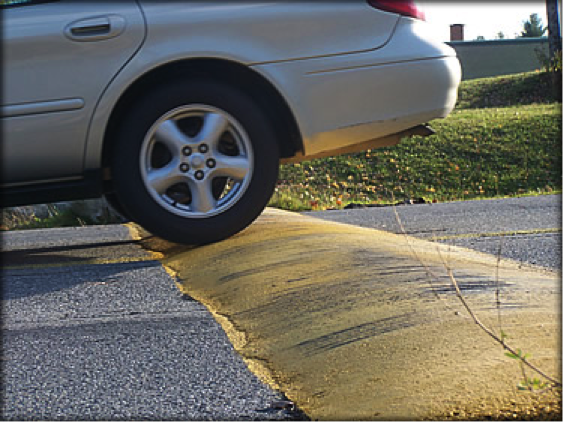
\includegraphics[scale=1]{speed-hump.png}
\caption{Speed Hump}\label{fig:speed-hump}
\end{figure}

\subsubsection{Cost and Considerations}

Factors to consider when creating chokers are to consult with the local fire and sanitation department before setting minimum width and to double check to make sure that the bicyclist safety and mobility are not diminished. Also when reducing two-lane street to one lane, the width of the travel way should not be wide enough for 2 cars to pass at the same time. This equals to the travel way not being wider than 4.9 meter, or 16 to 17 feet; by doing so, the effectiveness of the chocker is maximized \cite{walking-info-chokers}. The cost to create chokers varies depending on the site and landscape but most are along the lines of \$5,000 to \$20,000 (drainage representing a significant amount).